% !TeX root = ..\CYR2019.tex

\subsection{Sensors}
\label{sec:sensors}

Leakage currents, depletion voltage, CCE, etc.

\subsubsection{Leakage Current}
\label{sec:leakagecurrent}
%==============================================
%-------    Leakage Current:: Fluence Dependence -------------------------------------
%==============================================
\subsubsection*{Leakage Current: Fluence dependence}
%
After exposure to highly energetic particles having sufficient energy to produce so-called defect clusters (see e.g. \cite{2018-Moll-DD}), the radiation induced increase of the leakage current is proportional to the particle fluence and independent of the type, resistivity and impurity content of the used silicon material \cite{1999-Moll-current, 2013-Srour-DD}. This is shown in Fig.~\ref{fig:1999-Moll-phd-basic-leakage-fluence} for various silicon detectors \cite{1999-Moll-phd}.
The proportionality factor is called {\em current related damage factor $\alpha$} and is defined by 
\begin{equation}
\alpha =\frac{\Delta I}{V \phi_{eq}}
\end{equation}
where $\Delta I$ is the leakage current increase caused by irradiation, $V$ the volume contributing to the current and $\phi_{eq}$ the 1 MeV neutron equivalent particle fluence. The data shown in Fig.~\ref{fig:1999-Moll-phd-basic-leakage-fluence} result in a value of $\alpha$(80~min, 60$^\circ$C) = (3.99$\pm$0.03)$\times$10$^{-17}$ A/cm for the measurements taken at 20$^\circ$C. 
%---------------------------------------------------------------------
%-------  Figure: Leakage Current against Fluence
%---------------------------------------------------------------------
\begin{figure}[bth]
\centering
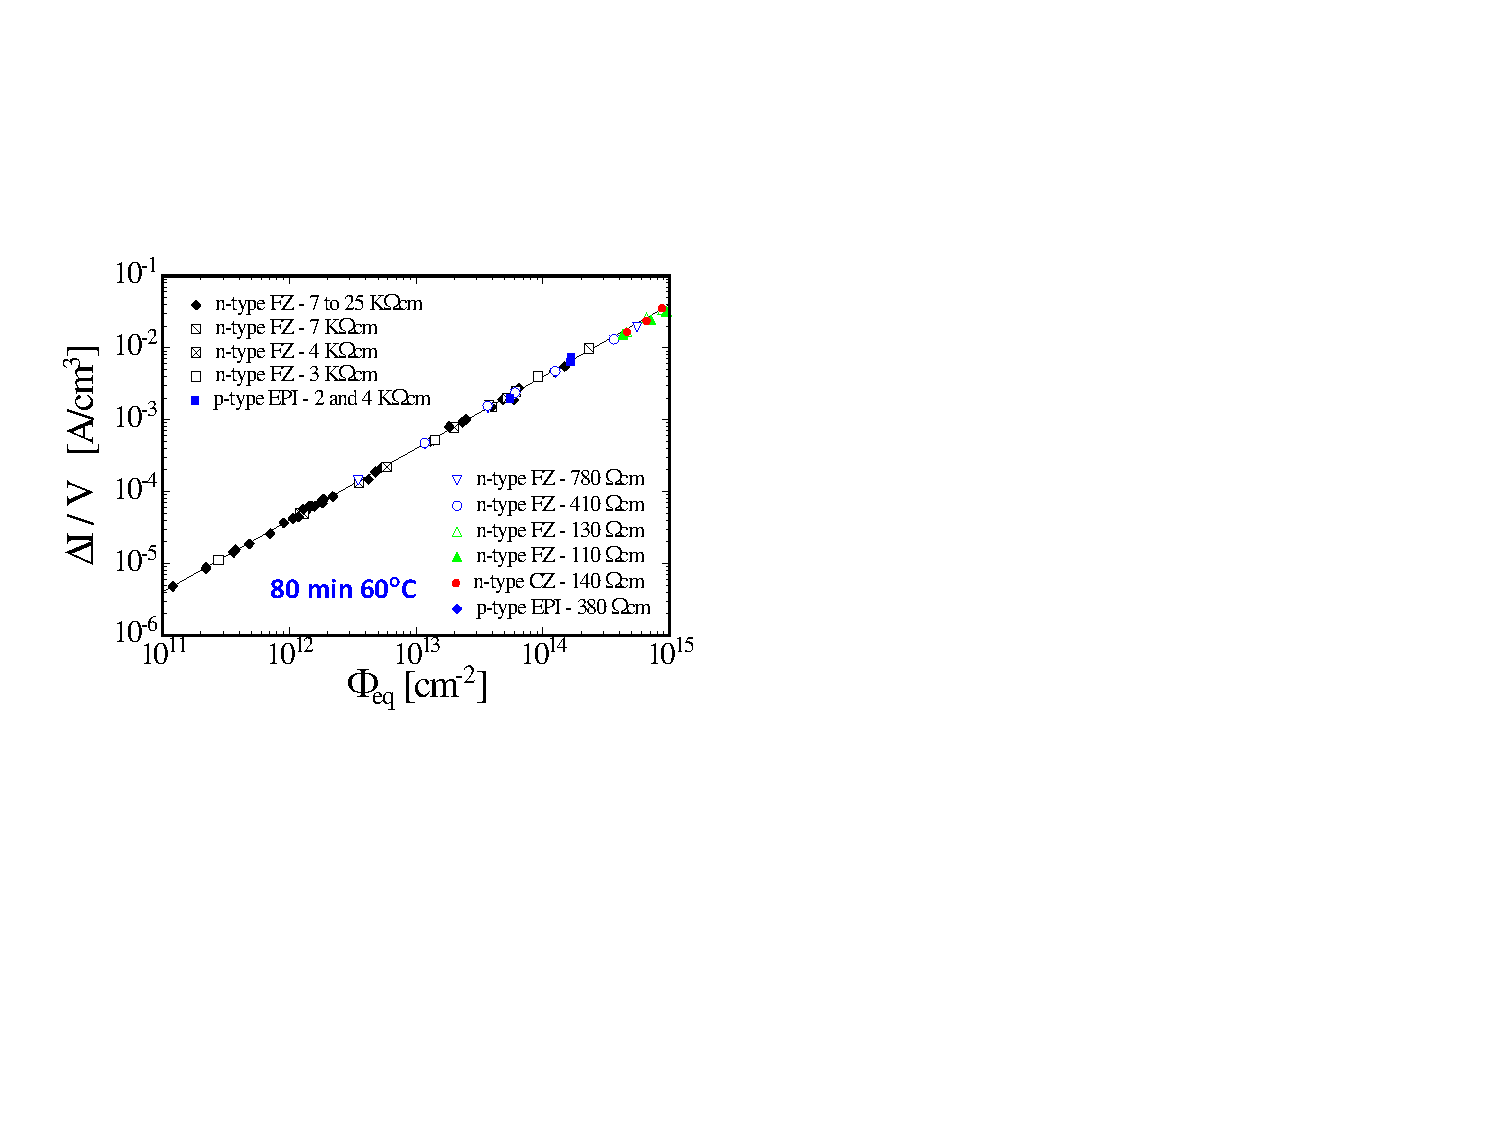
\includegraphics[width=0.6\linewidth]{figures/RadiationEffects/Sensors/1999-Moll-phd-basic-leakage-fluence.pdf}
\caption{
Radiation induced leakage current increase as function of particle fluence for various silicon detectors made from 
silicon materials produced by various process technologies with different resistivities and conduction type. The current was 
measured at room temperature (20$^\circ$C) after irradiation in a neutron field with 5.2 MeV mean energy and r a dedicated annealing of 80 min at 60$^\circ$C .
Figure taken from \cite{1999-Moll-phd}.}
\label{fig:1999-Moll-phd-basic-leakage-fluence}
\end{figure}
%---------------------------------------------------------------------

It shall be mentioned that for irradiations producing predominantly point defects (e.g. $^{60}$Co-gamma) a non-linear dependence on the particle fluence and a strong dependence on the impurity content are observed \cite{2003-Pintilie-gamma}. This case is not further treated here as in the LHC context the defect cluster induced leakage is the dominant one; more details regarding point-defect induced leakage can be found in \cite{2009-Pintilie-cluster}. 
%===================================================
%-------  Subsubsection: Leakage Current:: Temperature Dependence
%===================================================
\subsubsection*{Leakage Current: Temperature dependence}
The temperature dependence of the leakage current is dominated by the position of the energy levels in the band gap, their cross sections, their concentrations and the temperature dependence of the bandgap itself. 
The most efficient generation centers are the ones at the intrinsic energy level. In this case the  leakage current 
temperature dependence will follow the one of the intrinsic carrier concentration $n_i$. In a recent 
	work Chilingarov \cite{2013-Chilingarov-Tscaling} compared experimental results obtained on several different irradiated silicon particle detectors using the parameterization 
\begin{equation}
I(T) \propto T^2 \exp \left( - E_{eff}/2k_B T\right)
\end{equation}
and obtained a value of $E_{eff}$ = 1.214$\pm$0.014~eV. This value is presently the reference in the HEP 
community for temperature correction (scaling) of the leakage current. In practice this value translates into a reduction of the leakage current by  8\% to 10\% per degree centrigrade in the temperature range from RT to -20$^\circ$C.
%======================================================
%-------  Subsubsection: Leakage Current:: Annealing and Parameterization
%======================================================
\subsubsection*{Leakage Current: Annealing effects and parameterization}
The annealing behavior of the current related damage factor $\alpha$ after irradiation is displayed in Fig.~\ref{fig:1999-Moll-phd-basic-leakage-time} 
for various annealing temperatures ranging from 21$^\circ$C to 106$^\circ$C \cite{2002-Moll-micro-macro}. 
%---------------------------------------------------------------------
%-------  Figure: Leakage Current Annealing
%---------------------------------------------------------------------
\begin{figure}[!t]
\centering
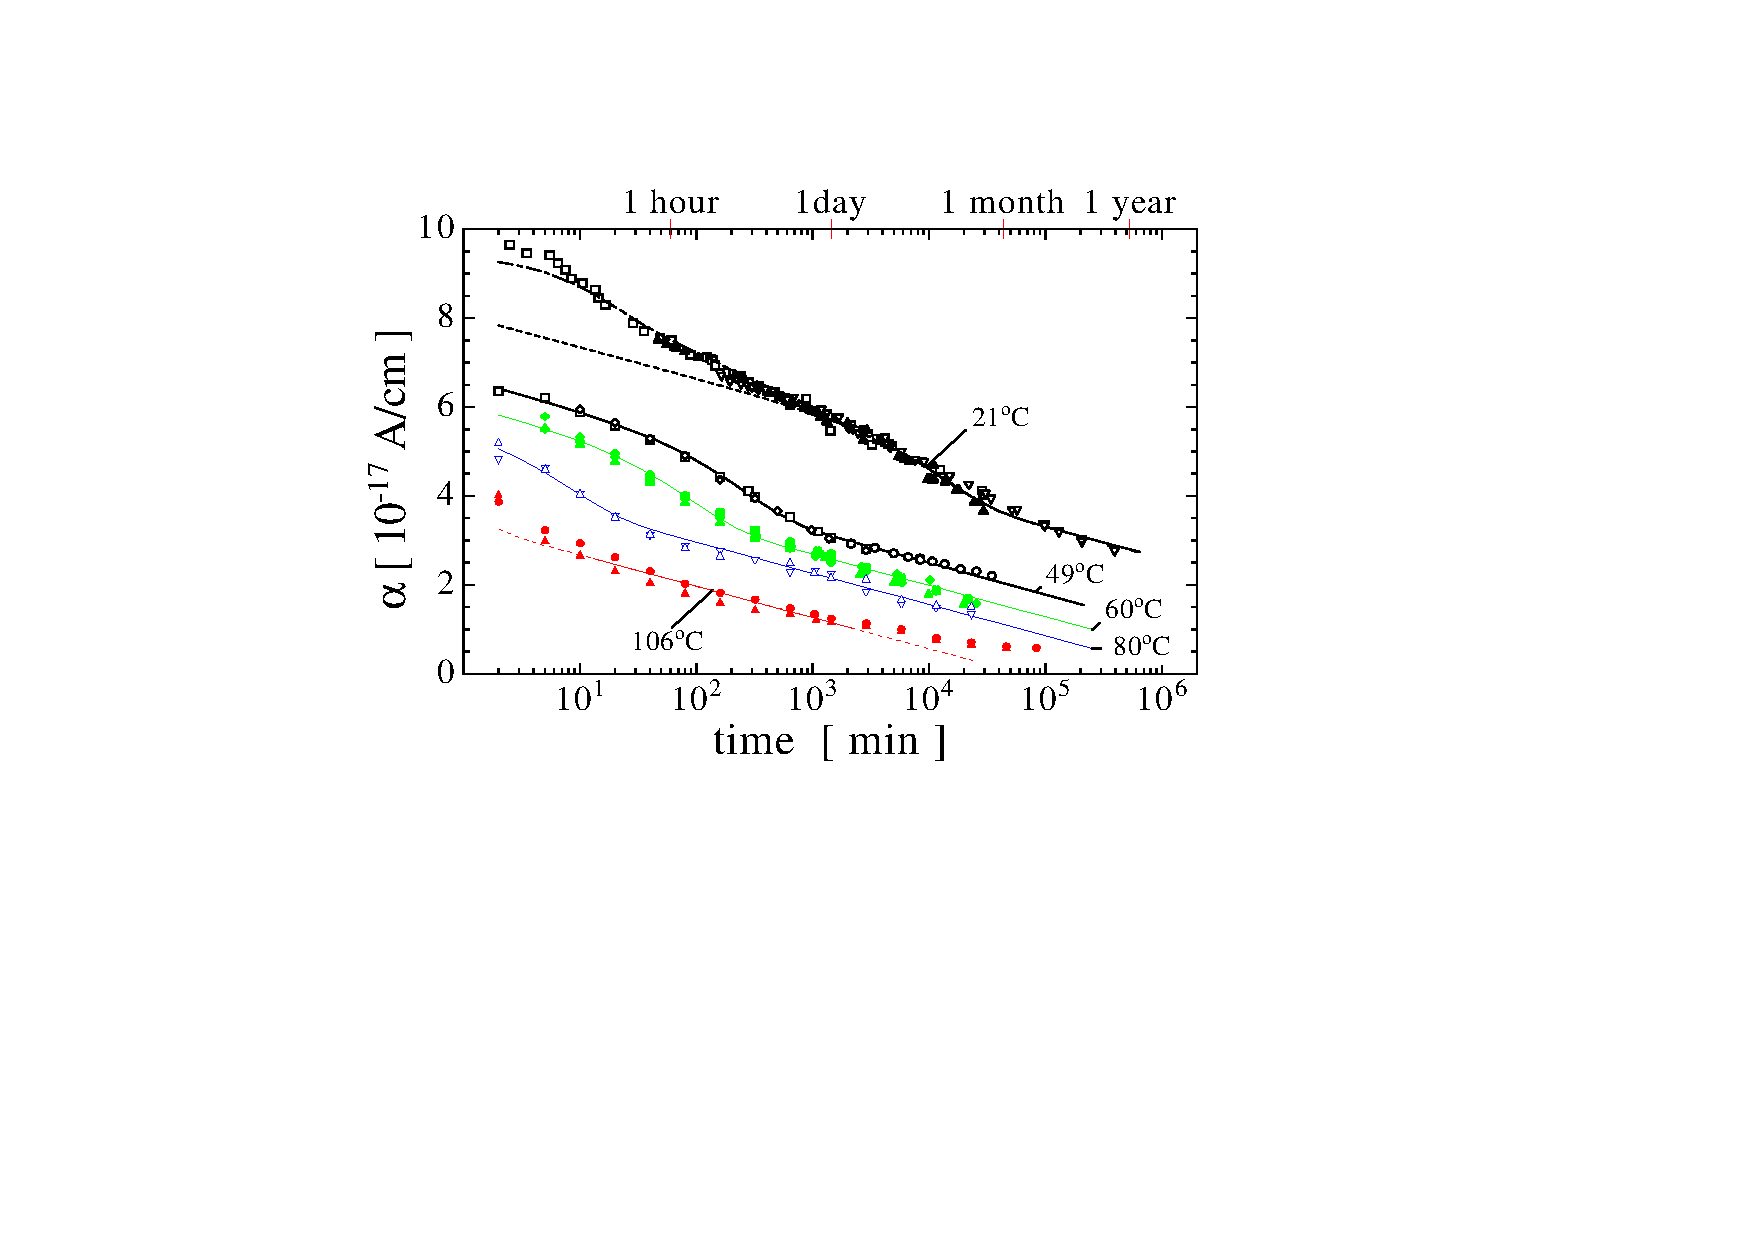
\includegraphics[width=0.8\linewidth]{figures/RadiationEffects/Sensors/1999-Moll-phd-basic-leakage-time.pdf}
\caption{
Current related damage rate $\alpha$ as a function of cumulated annealing time at different temperatures. Solid lines represent fits to the data (see text). Figure taken from \cite{2002-Moll-micro-macro}.}
\label{fig:1999-Moll-phd-basic-leakage-time}
\end{figure}
%---------------------------------------------------------------------
The annealing temperature is the temperature at which the samples are stored or heated to accelerate the defect reactions in the silicon 
bulk. This temperature shall not be confused with the measurement temperature of the leakage 
current which in the given example is 20$^\circ$C. The $\alpha$ value is 
continuously decreasing with increasing annealing time. 
%
In \cite{1999-Moll-phd, 2002-Moll-micro-macro} a parametrization of the data with an exponential and logarithmic term is proposed
\begin{equation}
\alpha = \alpha_1 \cdot \exp\left(-t/\tau_1 \right) + \alpha_0 -\alpha_2 \cdot \ln\left(t/t_0\right)    	  	
\end{equation}
and has been used in the figure to fit the data (solid lines). The complete parameter set ($\alpha_0$, $\alpha_1$, $\alpha_2$, $\tau_1$ and $t_0$) and a discussion on the physics meaning of the parameters can be found in \cite{1999-Moll-phd,2002-Moll-micro-macro}.
%======================================
%-------  Subsubsection: Space Charge - Depletion Voltage
%======================================
\subsubsection{Depletion Voltage - Space Charge - Effective Doping Concentration}
\label{sec:space_charge}
The radiation induced defects lead to a change in the effective space charge $N_{eff}$ that is reflected in a change of the depletion voltage $V_{dep}$ of silicon detectors. The depletion voltage $V_{dep}$ is given by
\begin{equation}
\label{eq:vdep_neff} 
V_{dep}= \frac{q\cdot\left|N_{eff}\right|\cdot d^2}{2 \cdot \epsilon\epsilon_0}
\end{equation}
where $d$ is the thickness of the device, $q$ the elementary charge, $\epsilon$ the relative permittivity of silicon and $\epsilon_0$ the vacuum permittivity. 
It shall be noted that Eq.~\ref{eq:vdep_neff} is assuming a constant space charge over the volume of the damaged detector, which is not always the case \cite{2002-Eremin-doublejunction}. Furthermore, the depletion voltage is usually determined from capacitance vs. voltage (CV) measurements at $\approx$ 10~kHz and a temperature between +20$^\circ$C and -20$^\circ$C depending on measurement limits set by the high leakage currents, while a dependence of the depletion voltage on the measurement frequency and temperature has been reported for damaged detectors \cite{2002-Campbell-vdep-ft}. It is thus understood that the following parameterizations give precise values for the prediction of the depletion voltage (i.e. the kink in the CV measurement of a diode), while the translation into $N_{eff}$ via Eq.~\ref{eq:vdep_neff} might be afflicted with systematic errors. 
It shall be mentioned that in highly irradiated detectors, contrary to undamaged detectors, the space charge is no longer identical to the free carrier concentration in thermal equilibrium. Results of characterization methods determining the free carrier densitity or the low voltage resistivity are therefore not easily correlated with the space charge determined from full depletion voltage.
%======================================================
%-------  Subsubsection: Vdep:: Fluence Dependence
%======================================================
\subsubsection*{Depletion Voltage: Fluence dependence}
\label{sec:vdep_phi}
 Fig.~\ref{fig:1999-Moll-phd-basic-vdep-phi} shows an example of the evolution of the effective space charge (i.e. depletion voltage) for an n-type sensor with particle fluence \cite{1992-Wunstorf-phd}. Before irradiation the sensor was of high resistivity n-type (Phosphorus doped) base material resulting in a positive space charge of some 10$^{11}$~cm$^{-3}$.
 %
Irradiation of the sensor results in the formation of negative space charge which compensates the initial positive space charge. With increasing particle fluence the net space charge decreases and reaches very low values corresponding to almost intrinsic silicon. 
 This point is called {\em type inversion} or {\em space charge sign inversion (SCSI)} as the space charge sign changes from positive to negative. Increasing the particle fluence beyond the SCSI point leads to more and more negative space charge values. The depletion voltage rises accordingly and eventually reaches values that cannot be applied to the detector any more without causing breakdown. The applied voltage will have to be kept below the depletion voltage and the detector is operated  “underdepleted”. \\
For high resistivity p-type sensors no “type inversion” is usually observed as the initial space charge is already negative before irradiation. It should however be mentioned that after neutron and charged hadron irradiations cases have been observed in non-standard silicon materials where type inversion occurs from negative to positive space charge \cite{1999-Moll-phd} or the effective space charge remains positive in n-type sensors up to very high particle fluences \cite{2006-Lindstrom-epi, 2011-Pacifico-mcz}.   
%---------------------------------------------------------------------
%-------  Figure: Depletion Voltage Fluence Dependence
%---------------------------------------------------------------------
\begin{figure}[bth]
\centering
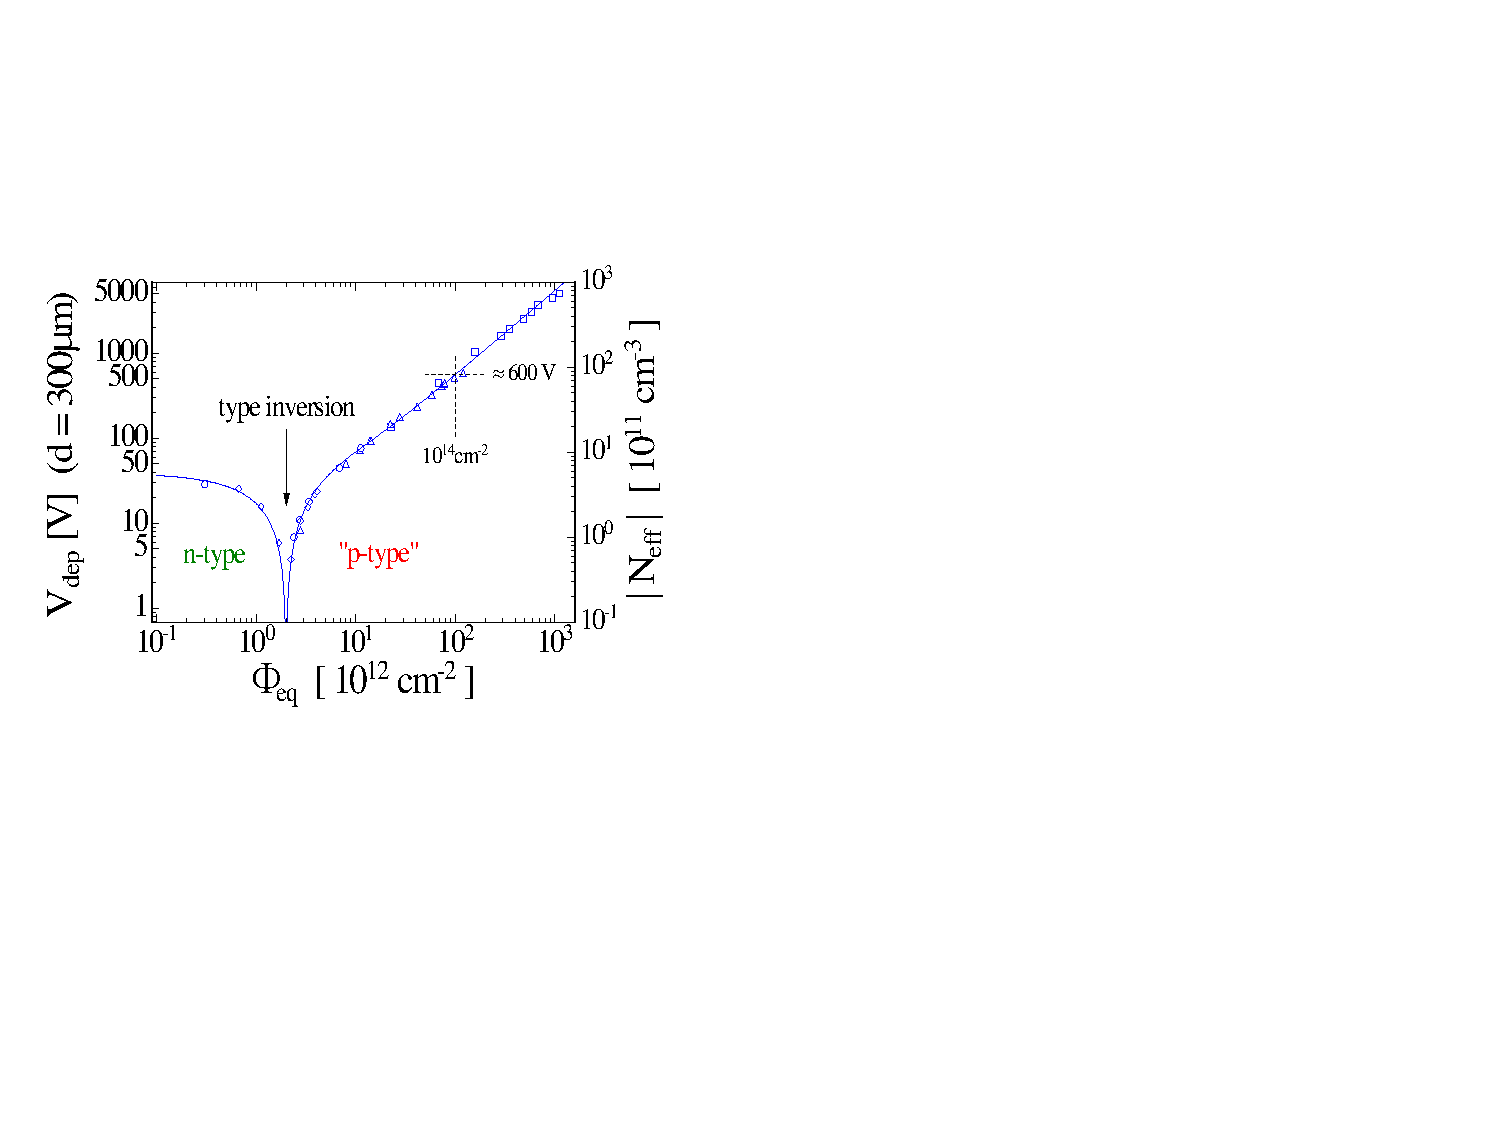
\includegraphics[width=0.6\linewidth]{figures/RadiationEffects/Sensors/1999-Moll-phd-basic-vdep-phi.pdf}
\caption{
Effective doping concentration (depletion voltage) as function of particle fluence for a standard FZ n-type silicon detector. Data were measured directly after exposure and are taken from \cite{1992-Wunstorf-phd}.}
\label{fig:1999-Moll-phd-basic-vdep-phi}
\end{figure}
%---------------------------------------------------------------------









\begin{thebibliography}{99}
\bibitem{2018-Moll-DD}
M. Moll, {\em Displacement Damage in Silicon Detectors for High Energy Physics}, 
\href{http://doi.org/10.1109/TNS.2018.2819506}{IEEE TNS, vol. 65, no. 8, pp. 1561-1582, Aug. 2018}.
%
\bibitem{1999-Moll-current}
M. Moll, E. Fretwurst and G. Lindstr{\"o}m, {\em Leakage current of hadron irradiated silicon detectors – material dependence}, 
\href{https://doi.org/10.1016/S0168-9002(98)01475-2}{NIMA 426, 87-93, 1999}.
%
\bibitem{2013-Srour-DD}
J. R. Srour and J. W. Palko,
{\em Displacement Damage Effects in Irradiated Semiconductor Devices}, 
\href{https://doi.org/10.1109/TNS.2013.2261316}{IEEE TNS, vol. 60, no.3,pp. 1740-1766,  June 2013}.
%
\bibitem{1999-Moll-phd}
    M. Moll, {\em Radiation damage in silicon particle detectors $-$ Microscopic defects and macroscopic properties $-$'}, \href{http://cds.cern.ch/record/425274}{PhD thesis: Hamburg University, 1999}.
%    
\bibitem{2003-Pintilie-gamma}
I.~Pintilie et al., 
{\em Results on defects induced by $^{60}${Co} gamma irradiation in standard and oxygen-enriched silicon},
\href{https://doi.org/10.1016/j.nima.2003.08.079}{NIMA 514, 18 - 24, 2003}.
%
\bibitem{2009-Pintilie-cluster}
I.~Pintilie et al., {\em Radiation-induced point- and cluster-related defects with strong impact on damage properties of silicon detectors},
\href{https://doi.org/10.1016/j.nima.2009.09.065}{NIMA, 611, 52 - 68, 2009}.
%
\bibitem{2013-Chilingarov-Tscaling}
A.~Chilingarov, {\em Temperature dependence of the current generated in {Si} bulk},
\href{https://doi.org/10.1088/1748-0221/8/10/P10003}{JINST, vol.8, no.10, P10003, 2013}.
%
\bibitem{2002-Moll-micro-macro}
M Moll et al., 
{\em Relation between microscopic defects and macroscopic changes in silicon detector properties after hadron irradiation}, \href{https://doi.org/10.1016/S0168-583X(01)00866-7}{NIMB 186, pp. 100 - 110, 2002}
%
\bibitem{1992-Wunstorf-phd}
 R.~Wunstorf, {\em Systematische Untersuchung zur Strahlenresistenz von Silizium-Detektoren
         f{\"u}r die Verwendung in Hochenergiephysik-Experimenten}, 
\href{https://cds.cern.ch/record/243081}{PhD thesis: Hamburg University, 1992}.
%
\bibitem{2006-Lindstrom-epi}
G. Lindstr{\"o}m et al., {\em Radiation tolerance of epitaxial silicon detectors at very large proton fluences},
\href{https://doi.org/10.1016/j.nima.2005.10.103}{NIMA 556, pp 451-458, 2006}.
%
\bibitem{2011-Pacifico-mcz}
N.~Pacifico et al., {\em Characterization of proton and neutron irradiated low resistivity p-on-n magnetic Czochralski ministrip sensors and diodes}, 
\href{https://doi.org/10.1016/j.nima.2011.03.026}{NIMA 658, pp 55 - 60, 2011}.
\end{thebibliography}
